\documentclass[]{article}
\usepackage{lmodern}
\usepackage{amssymb,amsmath}
\usepackage{ifxetex,ifluatex}
\usepackage{fixltx2e} % provides \textsubscript
\ifnum 0\ifxetex 1\fi\ifluatex 1\fi=0 % if pdftex
  \usepackage[T1]{fontenc}
  \usepackage[utf8]{inputenc}
\else % if luatex or xelatex
  \ifxetex
    \usepackage{mathspec}
  \else
    \usepackage{fontspec}
  \fi
  \defaultfontfeatures{Ligatures=TeX,Scale=MatchLowercase}
\fi
% use upquote if available, for straight quotes in verbatim environments
\IfFileExists{upquote.sty}{\usepackage{upquote}}{}
% use microtype if available
\IfFileExists{microtype.sty}{%
\usepackage{microtype}
\UseMicrotypeSet[protrusion]{basicmath} % disable protrusion for tt fonts
}{}
\usepackage[margin=1in]{geometry}
\usepackage{hyperref}
\hypersetup{unicode=true,
            pdftitle={Example Pretty XTable},
            pdfauthor={Keaton Stagaman},
            pdfborder={0 0 0},
            breaklinks=true}
\urlstyle{same}  % don't use monospace font for urls
\usepackage{color}
\usepackage{fancyvrb}
\newcommand{\VerbBar}{|}
\newcommand{\VERB}{\Verb[commandchars=\\\{\}]}
\DefineVerbatimEnvironment{Highlighting}{Verbatim}{commandchars=\\\{\}}
% Add ',fontsize=\small' for more characters per line
\usepackage{framed}
\definecolor{shadecolor}{RGB}{248,248,248}
\newenvironment{Shaded}{\begin{snugshade}}{\end{snugshade}}
\newcommand{\KeywordTok}[1]{\textcolor[rgb]{0.13,0.29,0.53}{\textbf{{#1}}}}
\newcommand{\DataTypeTok}[1]{\textcolor[rgb]{0.13,0.29,0.53}{{#1}}}
\newcommand{\DecValTok}[1]{\textcolor[rgb]{0.00,0.00,0.81}{{#1}}}
\newcommand{\BaseNTok}[1]{\textcolor[rgb]{0.00,0.00,0.81}{{#1}}}
\newcommand{\FloatTok}[1]{\textcolor[rgb]{0.00,0.00,0.81}{{#1}}}
\newcommand{\ConstantTok}[1]{\textcolor[rgb]{0.00,0.00,0.00}{{#1}}}
\newcommand{\CharTok}[1]{\textcolor[rgb]{0.31,0.60,0.02}{{#1}}}
\newcommand{\SpecialCharTok}[1]{\textcolor[rgb]{0.00,0.00,0.00}{{#1}}}
\newcommand{\StringTok}[1]{\textcolor[rgb]{0.31,0.60,0.02}{{#1}}}
\newcommand{\VerbatimStringTok}[1]{\textcolor[rgb]{0.31,0.60,0.02}{{#1}}}
\newcommand{\SpecialStringTok}[1]{\textcolor[rgb]{0.31,0.60,0.02}{{#1}}}
\newcommand{\ImportTok}[1]{{#1}}
\newcommand{\CommentTok}[1]{\textcolor[rgb]{0.56,0.35,0.01}{\textit{{#1}}}}
\newcommand{\DocumentationTok}[1]{\textcolor[rgb]{0.56,0.35,0.01}{\textbf{\textit{{#1}}}}}
\newcommand{\AnnotationTok}[1]{\textcolor[rgb]{0.56,0.35,0.01}{\textbf{\textit{{#1}}}}}
\newcommand{\CommentVarTok}[1]{\textcolor[rgb]{0.56,0.35,0.01}{\textbf{\textit{{#1}}}}}
\newcommand{\OtherTok}[1]{\textcolor[rgb]{0.56,0.35,0.01}{{#1}}}
\newcommand{\FunctionTok}[1]{\textcolor[rgb]{0.00,0.00,0.00}{{#1}}}
\newcommand{\VariableTok}[1]{\textcolor[rgb]{0.00,0.00,0.00}{{#1}}}
\newcommand{\ControlFlowTok}[1]{\textcolor[rgb]{0.13,0.29,0.53}{\textbf{{#1}}}}
\newcommand{\OperatorTok}[1]{\textcolor[rgb]{0.81,0.36,0.00}{\textbf{{#1}}}}
\newcommand{\BuiltInTok}[1]{{#1}}
\newcommand{\ExtensionTok}[1]{{#1}}
\newcommand{\PreprocessorTok}[1]{\textcolor[rgb]{0.56,0.35,0.01}{\textit{{#1}}}}
\newcommand{\AttributeTok}[1]{\textcolor[rgb]{0.77,0.63,0.00}{{#1}}}
\newcommand{\RegionMarkerTok}[1]{{#1}}
\newcommand{\InformationTok}[1]{\textcolor[rgb]{0.56,0.35,0.01}{\textbf{\textit{{#1}}}}}
\newcommand{\WarningTok}[1]{\textcolor[rgb]{0.56,0.35,0.01}{\textbf{\textit{{#1}}}}}
\newcommand{\AlertTok}[1]{\textcolor[rgb]{0.94,0.16,0.16}{{#1}}}
\newcommand{\ErrorTok}[1]{\textcolor[rgb]{0.64,0.00,0.00}{\textbf{{#1}}}}
\newcommand{\NormalTok}[1]{{#1}}
\usepackage{graphicx,grffile}
\makeatletter
\def\maxwidth{\ifdim\Gin@nat@width>\linewidth\linewidth\else\Gin@nat@width\fi}
\def\maxheight{\ifdim\Gin@nat@height>\textheight\textheight\else\Gin@nat@height\fi}
\makeatother
% Scale images if necessary, so that they will not overflow the page
% margins by default, and it is still possible to overwrite the defaults
% using explicit options in \includegraphics[width, height, ...]{}
\setkeys{Gin}{width=\maxwidth,height=\maxheight,keepaspectratio}
\IfFileExists{parskip.sty}{%
\usepackage{parskip}
}{% else
\setlength{\parindent}{0pt}
\setlength{\parskip}{6pt plus 2pt minus 1pt}
}
\setlength{\emergencystretch}{3em}  % prevent overfull lines
\providecommand{\tightlist}{%
  \setlength{\itemsep}{0pt}\setlength{\parskip}{0pt}}
\setcounter{secnumdepth}{0}
% Redefines (sub)paragraphs to behave more like sections
\ifx\paragraph\undefined\else
\let\oldparagraph\paragraph
\renewcommand{\paragraph}[1]{\oldparagraph{#1}\mbox{}}
\fi
\ifx\subparagraph\undefined\else
\let\oldsubparagraph\subparagraph
\renewcommand{\subparagraph}[1]{\oldsubparagraph{#1}\mbox{}}
\fi
\usepackage{subfig}
\usepackage{graphicx}
\usepackage{graphics}
\usepackage{xcolor}
\usepackage{hyperref}
\usepackage[hypcap]{caption}
\usepackage{adjustbox}
\usepackage{float}
\usepackage[utf8]{inputenc}
\maxdeadcycles=1000

%%% Use protect on footnotes to avoid problems with footnotes in titles
\let\rmarkdownfootnote\footnote%
\def\footnote{\protect\rmarkdownfootnote}

%%% Change title format to be more compact
\usepackage{titling}

% Create subtitle command for use in maketitle
\newcommand{\subtitle}[1]{
  \posttitle{
    \begin{center}\large#1\end{center}
    }
}

\setlength{\droptitle}{-2em}
  \title{Example Pretty XTable}
  \pretitle{\vspace{\droptitle}\centering\huge}
  \posttitle{\par}
  \author{Keaton Stagaman}
  \preauthor{\centering\large\emph}
  \postauthor{\par}
  \predate{\centering\large\emph}
  \postdate{\par}
  \date{July 7, 2016}

\begin{document}
\maketitle

\subsection{Load libraries and source
files}\label{load-libraries-and-source-files}

\begin{Shaded}
\begin{Highlighting}[]
\KeywordTok{library}\NormalTok{(qdap)}
\KeywordTok{library}\NormalTok{(ggfortify)}
\KeywordTok{library}\NormalTok{(ggplot2)}
\KeywordTok{theme_set}\NormalTok{(}\KeywordTok{theme_bw}\NormalTok{())}
\KeywordTok{source}\NormalTok{(}\StringTok{"../xtable_summary.R"}\NormalTok{)}
\end{Highlighting}
\end{Shaded}

\subsection{Data plot with regression
line}\label{data-plot-with-regression-line}

\begin{Shaded}
\begin{Highlighting}[]
\KeywordTok{ggplot}\NormalTok{(mtcars, }\KeywordTok{aes}\NormalTok{(}\DataTypeTok{x=}\NormalTok{disp, }\DataTypeTok{y=}\NormalTok{mpg)) +}\StringTok{ }
\StringTok{    }\KeywordTok{geom_point}\NormalTok{(}\KeywordTok{aes}\NormalTok{(}\DataTypeTok{color=}\KeywordTok{as.factor}\NormalTok{(cyl)), }\DataTypeTok{size=}\DecValTok{3}\NormalTok{) +}\StringTok{ }
\StringTok{    }\KeywordTok{scale_color_brewer}\NormalTok{(}\DataTypeTok{name=}\StringTok{"Cylinders"}\NormalTok{, }\DataTypeTok{palette=}\StringTok{"Accent"}\NormalTok{) +}\StringTok{ }
\StringTok{    }\KeywordTok{stat_smooth}\NormalTok{(}\DataTypeTok{method=}\StringTok{"lm"}\NormalTok{) +}\StringTok{ }
\StringTok{    }\KeywordTok{labs}\NormalTok{(}\DataTypeTok{x=}\StringTok{"Displacement"}\NormalTok{, }\DataTypeTok{y=}\StringTok{"Miles per Gallon"}\NormalTok{)}
\end{Highlighting}
\end{Shaded}

\begin{figure}[htbp]
\centering
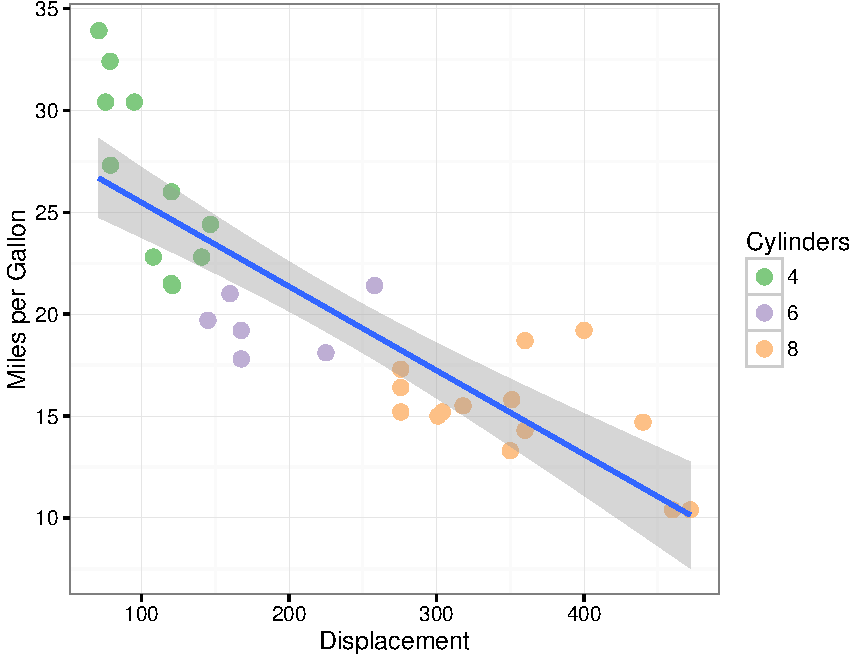
\includegraphics{example_files/figure-latex/mtcars_plot-1.pdf}
\caption{Car distance by speed with regression line}
\end{figure}

\subsection{Linear model calculation}\label{linear-model-calculation}

\begin{Shaded}
\begin{Highlighting}[]
\NormalTok{mtcars.lm <-}\StringTok{ }\KeywordTok{lm}\NormalTok{(mpg ~}\StringTok{ }\NormalTok{disp*cyl, }\DataTypeTok{data=}\NormalTok{mtcars)}
\KeywordTok{xtable.summary}\NormalTok{(}\DataTypeTok{model.obj=}\NormalTok{mtcars.lm, }
               \DataTypeTok{file.id=}\StringTok{"mtcars"}\NormalTok{, }
               \DataTypeTok{alt.factor.names=}\KeywordTok{mgsub}\NormalTok{(}\KeywordTok{c}\NormalTok{(}\StringTok{"disp"}\NormalTok{, }\StringTok{"cyl"}\NormalTok{), }
                                      \KeywordTok{c}\NormalTok{(}\StringTok{"Displacement"}\NormalTok{, }\StringTok{"Cylinders"}\NormalTok{), }
                                      \KeywordTok{attributes}\NormalTok{(mtcars.lm$terms)$term.labels))}
\end{Highlighting}
\end{Shaded}

\begin{table}[h!]
\captionsetup[subtable]{labelformat=empty}
\centering
\subfloat[]{\label{tab:mtcars_lm-a}{% latex table generated in R 3.3.1 by xtable 1.8-2 package
% Fri Jul  8 14:09:29 2016
\begin{tabular}{rrrrr}
  \hline
 & Estimate & Std. Error & t value & Pr(>|t|) \\ 
  \hline
\textbf{(Intercept)} & 49.0372 & 5.0046 & 9.80 & \textbf{1.51e-10} \\ 
  \textbf{Displacement} & -0.1455 & 0.0400 & -3.64 & \textbf{0.0011} \\ 
  \textbf{Cylinders} & -3.4052 & 0.8402 & -4.05 & \textbf{0.000365} \\ 
  \textbf{Displacement:Cylinders} & 0.0159 & 0.0049 & 3.20 & \textbf{0.00337} \\ 
   \hline
\end{tabular}
}}\quad
\subfloat[]{\label{tab:mtcars_lm-b}{% latex table generated in R 3.3.1 by xtable 1.8-2 package
% Fri Jul  8 14:09:29 2016
\begin{tabular}{rrrrr}
  \hline
D.f. & Residual Std. Error & $R^2$ & Adjusted $R^2$ & $p$-value \\ 
  \hline
 28 & 2.66 & 0.82 & 0.81 & 0.00 \\ 
   \hline
\end{tabular}
}}
\caption{Linear model for Miles per Gallon by Displacement and Number of Cylinders}
\label{tab:mtcars_lm}
\end{table}

\subsection{Factor analysis}\label{factor-analysis}

\begin{Shaded}
\begin{Highlighting}[]
\NormalTok{factanal1 <-}\StringTok{ }\KeywordTok{factanal}\NormalTok{(mtcars, }\DataTypeTok{factors=}\DecValTok{1}\NormalTok{, }\DataTypeTok{scores=}\StringTok{"regression"}\NormalTok{)}
\KeywordTok{paste}\NormalTok{(}\StringTok{"1 factor p-val:"}\NormalTok{, factanal1$PVAL)}
\end{Highlighting}
\end{Shaded}

\begin{verbatim}
## [1] "1 factor p-val: 1.49621956585337e-17"
\end{verbatim}

\begin{Shaded}
\begin{Highlighting}[]
\NormalTok{factanal2 <-}\StringTok{ }\KeywordTok{factanal}\NormalTok{(mtcars, }\DataTypeTok{factors=}\DecValTok{2}\NormalTok{, }\DataTypeTok{scores=}\StringTok{"regression"}\NormalTok{)}
\KeywordTok{paste}\NormalTok{(}\StringTok{"2 factor p-val:"}\NormalTok{, factanal2$PVAL)}
\end{Highlighting}
\end{Shaded}

\begin{verbatim}
## [1] "2 factor p-val: 0.000404750976192007"
\end{verbatim}

\begin{Shaded}
\begin{Highlighting}[]
\NormalTok{factanal3 <-}\StringTok{ }\KeywordTok{factanal}\NormalTok{(mtcars, }\DataTypeTok{factors=}\DecValTok{3}\NormalTok{, }\DataTypeTok{scores=}\StringTok{"regression"}\NormalTok{)}
\KeywordTok{paste}\NormalTok{(}\StringTok{"3 factor p-val:"}\NormalTok{, factanal3$PVAL)}
\end{Highlighting}
\end{Shaded}

\begin{verbatim}
## [1] "3 factor p-val: 0.205192300877265"
\end{verbatim}

\begin{Shaded}
\begin{Highlighting}[]
\KeywordTok{xtable.summary}\NormalTok{(}\DataTypeTok{model.obj=}\NormalTok{factanal3, }
               \DataTypeTok{file.id=}\StringTok{"mtcars"}\NormalTok{, }
               \DataTypeTok{cutoff=}\FloatTok{0.4}\NormalTok{, }
               \DataTypeTok{alt.factor.names=}\KeywordTok{c}\NormalTok{(}\StringTok{"Miles/Gal"}\NormalTok{, }
                                  \StringTok{"No. Cylinders"}\NormalTok{, }
                                  \StringTok{"Displacement"}\NormalTok{, }
                                  \StringTok{"Horsepower"}\NormalTok{, }
                                  \StringTok{"Rear Axle Ratio"}\NormalTok{, }
                                  \StringTok{"Weight"}\NormalTok{, }
                                  \StringTok{"1/4 mile time"}\NormalTok{, }
                                  \StringTok{"V/S"}\NormalTok{, }
                                  \StringTok{"Transmission"}\NormalTok{, }
                                  \StringTok{"No. Fwd Gears"}\NormalTok{, }
                                  \StringTok{"No. Carburetors"}\NormalTok{))}
\end{Highlighting}
\end{Shaded}

\begin{table}[h!]
\captionsetup[subtable]{labelformat=empty}
\centering
\subfloat[]{\label{tab:mtcars_fa-a}{% latex table generated in R 3.3.1 by xtable 1.8-2 package
% Fri Jul  8 14:09:29 2016
\begin{tabular}{rrrrrrrrrrrr}
  \hline
 & mpg & cyl & disp & hp & drat & wt & qsec & vs & am & gear & carb \\ 
  \hline
Uniquenesses & 0.13 & 0.06 & 0.09 & 0.13 & 0.29 & 0.06 & 0.05 & 0.22 & 0.21 & 0.12 & 0.16 \\ 
   \hline
\end{tabular}
}}\quad
\subfloat[]{\label{tab:mtcars_fa-b}{% latex table generated in R 3.3.1 by xtable 1.8-2 package
% Fri Jul  8 14:09:29 2016
\begin{tabular}{rlll}
  \hline
 & Factor1 & Factor2 & Factor3 \\ 
  \hline
Miles/Gal & \textbf{0.64} & \textbf{-0.48} & \textbf{-0.47} \\ 
  No. Cylinders & \textbf{-0.62} & \textbf{0.7} & 0.26 \\ 
  Displacement & \textbf{-0.72} & \textbf{0.54} & 0.32 \\ 
  Horsepower & -0.29 & \textbf{0.72} & \textbf{0.51} \\ 
  Rear Axle Ratio & \textbf{0.8} & -0.24 & -0.068 \\ 
  Weight & \textbf{-0.78} & 0.25 & \textbf{0.52} \\ 
  1/4 mile time & -0.18 & \textbf{-0.95} & -0.15 \\ 
  V/S & 0.3 & \textbf{-0.8} & -0.2 \\ 
  Transmission & \textbf{0.88} & 0.088 & -0.093 \\ 
  No. Fwd Gears & \textbf{0.91} & 0.021 & 0.22 \\ 
  No. Carburetors & 0.11 & \textbf{0.56} & \textbf{0.72} \\ 
   \hline
\end{tabular}
}}\quad
\subfloat[]{\label{tab:mtcars_fa-c}{% latex table generated in R 3.3.1 by xtable 1.8-2 package
% Fri Jul  8 14:09:29 2016
\begin{tabular}{rrrr}
  \hline
 & Factor1 & Factor2 & Factor3 \\ 
  \hline
SS Loadings & 4.38 & 3.52 & 1.58 \\ 
  Proportion Var. & 0.40 & 0.32 & 0.14 \\ 
  Cumulative Var. & 0.40 & 0.72 & 0.86 \\ 
   \hline
\end{tabular}
}}
\caption{Factor analysis results}
\label{tab:mtcars_fa}
\end{table}

\subsection{Model Selection}\label{model-selection}

\begin{Shaded}
\begin{Highlighting}[]
\NormalTok{m0 <-}\StringTok{ }\KeywordTok{lm}\NormalTok{(mpg ~}\StringTok{ }\NormalTok{cyl, }\DataTypeTok{data=}\NormalTok{mtcars)}
\NormalTok{m1 <-}\StringTok{ }\KeywordTok{lm}\NormalTok{(mpg ~}\StringTok{ }\NormalTok{cyl +}\StringTok{ }\NormalTok{disp, }\DataTypeTok{data=}\NormalTok{mtcars)}
\NormalTok{m2 <-}\StringTok{ }\KeywordTok{lm}\NormalTok{(mpg ~}\StringTok{ }\NormalTok{cyl +}\StringTok{ }\NormalTok{disp +}\StringTok{ }\NormalTok{hp, }\DataTypeTok{data=}\NormalTok{mtcars)}
\NormalTok{m3 <-}\StringTok{ }\KeywordTok{lm}\NormalTok{(mpg ~}\StringTok{ }\NormalTok{cyl +}\StringTok{ }\NormalTok{disp +}\StringTok{ }\NormalTok{hp +}\StringTok{ }\NormalTok{drat, }\DataTypeTok{data=}\NormalTok{mtcars)}
\NormalTok{m4 <-}\StringTok{ }\KeywordTok{lm}\NormalTok{(mpg ~}\StringTok{ }\NormalTok{cyl +}\StringTok{ }\NormalTok{disp +}\StringTok{ }\NormalTok{hp +}\StringTok{ }\NormalTok{drat +}\StringTok{ }\NormalTok{wt, }\DataTypeTok{data=}\NormalTok{mtcars)}
\NormalTok{mtcars.anova <-}\StringTok{ }\KeywordTok{anova}\NormalTok{(m0, m1, m2, m3, m4)}
\KeywordTok{xtable.summary}\NormalTok{(}\DataTypeTok{model.obj=}\NormalTok{mtcars.anova, }
               \DataTypeTok{file.id=}\StringTok{"mtcars"}\NormalTok{,}
               \DataTypeTok{alt.models.text=}\KeywordTok{mgsub}\NormalTok{(}\KeywordTok{c}\NormalTok{(}\StringTok{"mpg"}\NormalTok{, }\StringTok{"cyl"}\NormalTok{, }\StringTok{"disp"}\NormalTok{, }\StringTok{"hp"}\NormalTok{, }\StringTok{"drat"}\NormalTok{, }\StringTok{"wt"}\NormalTok{),}
                                     \KeywordTok{c}\NormalTok{(}\StringTok{"Miles/Gal"}\NormalTok{,}
                                       \StringTok{"No. Cylinders"}\NormalTok{,}
                                       \StringTok{"Displacement"}\NormalTok{,}
                                       \StringTok{"Horsepower"}\NormalTok{,}
                                       \StringTok{"Rear Axle Ratio"}\NormalTok{,}
                                       \StringTok{"Weight"}\NormalTok{),}
                                     \KeywordTok{attributes}\NormalTok{(mtcars.anova)$heading[}\DecValTok{2}\NormalTok{],}
                                     \DataTypeTok{trim=}\OtherTok{FALSE}\NormalTok{))}
\end{Highlighting}
\end{Shaded}

\begin{table}[h!]
\captionsetup[subtable]{labelformat=empty}
\centering
\subfloat[]{\label{tab:mtcars_anova-a}{% latex table generated in R 3.3.1 by xtable 1.8-2 package
% Fri Jul  8 14:09:29 2016
\begin{tabular}{l}
  \hline
Analysis of Variance Table \\ 
  \hline
Model 1: Miles/Gal \textasciitilde No. Cylinders \\ 
  Model 2: Miles/Gal \textasciitilde No. Cylinders + Displacement \\ 
  Model 3: Miles/Gal \textasciitilde No. Cylinders + Displacement + Horsepower \\ 
  Model 4: Miles/Gal \textasciitilde No. Cylinders + Displacement + Horsepower + Rear Axle Ratio \\ 
  Model 5: Miles/Gal \textasciitilde No. Cylinders + Displacement + Horsepower + Rear Axle Ratio + Weight \\ 
   \hline
\end{tabular}
}}\quad
\subfloat[]{\label{tab:mtcars_anova-b}{% latex table generated in R 3.3.1 by xtable 1.8-2 package
% Fri Jul  8 14:09:29 2016
\begin{tabular}{lrrrrrr}
  \hline
 & Res. D.f. & RSS & D.f. & Sum. of Sq. & $F$ & Pr($>F$) \\ 
  \hline
1 & 30 & 308.33 &  &  &  &  \\ 
  \textbf{2} & 29 & 270.74 & 1 & 37.59 & 5.84 & \textbf{0.023} \\ 
  3 & 28 & 261.37 & 1 & 9.37 & 1.46 & 0.239 \\ 
  4 & 27 & 244.90 & 1 & 16.47 & 2.56 & 0.122 \\ 
  \textbf{5} & 26 & 167.43 & 1 & 77.48 & 12.03 & \textbf{0.00184} \\ 
   \hline
\end{tabular}
}}
\caption{Model Selection for Factors Contributing to Miles per Gallon}
\label{tab:mtcars_anova}
\end{table}


\end{document}
